\chapter{الكيمياء غير العضوية الحيوية}\label{ch:b3:bioinorganic}

دمنا أحمر بسبب الحديد؛ أما دم سرطان حدوة الحصان فعديم اللون في
أوردته ويصير أزرق في الهواء، لأنه يحمل الأكسجين على النحاس. وتستعمل الحياة
حفنة من الأيونات الفلزية للمهام التي لا تقدر عليها أي مجموعة عضوية: ربط الأكسجين
ربطًا عكوسًا، ونقل إلكترونات مفردة، وشطر الماء، واختزال النيتروجين،
وجعل جزيء ماء حمضيًا بما يكفي لمهاجمة ثنائي أكسيد الكربون. ويقرأ هذا الفصل
تلك المهام بأدوات كيمياء التناسق: \omterm{def:b3:bioinorganic:hsab}{الأحماض القاسية} واللينة،
ومجالات الربائط وحالات السبين، والتوازنات وقوانين السرعة، وينتهي
بالفلزات المستعملة أدويةً.

\begin{recall}
عالج مجلد السنة الثانية الأحماض الأمينية $\alpha$ والسلاسل الجانبية والببتيدات، والقواعد النووية
والنيوكليوتيدات، ومعقدات التناسق، ومجالات الربائط، والسبين العالي والمنخفض، 
والمحبات للنواة والمحبات للإلكترونات القاسية واللينة؛ وعالج مجلد السنة الأولى ثوابت التعقيد
وسلّم pL. وأعطى \cref{ch:b3:complex-spectra-magnetism} 
و\cref{ch:b3:complex-mechanisms} الأطياف ونظرية ماركوس وتميّه
السيسبلاتين، و\cref{ch:b3:complex-kinetics} حركية ميكايليس--منتن، 
و\cref{ch:b3:advanced-nmr} زمن الاسترخاء $T_1$.
\end{recall}

\begin{omfigure}
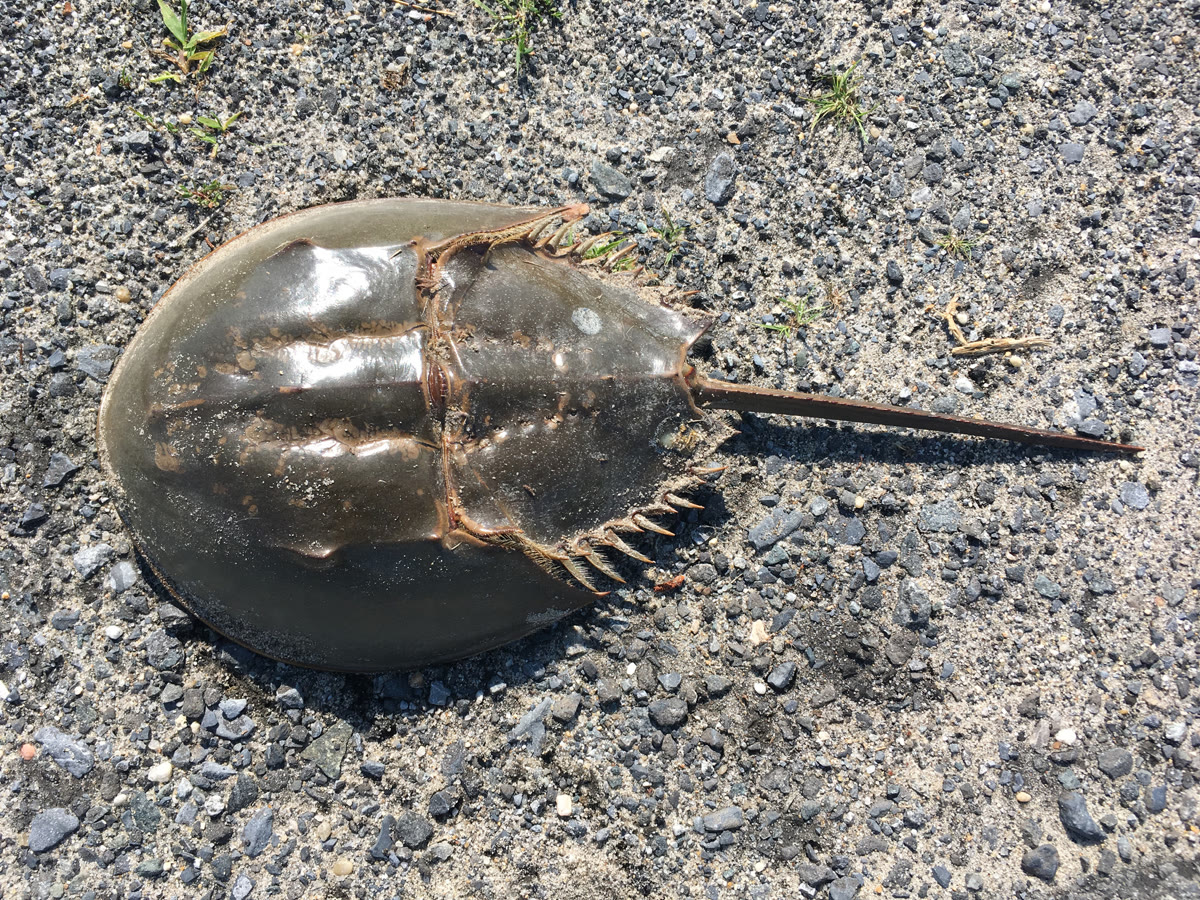
\includegraphics[width=0.5\linewidth]{images/book4/horseshoe-crab.jpg}

{\small سرطان حدوة الحصان الأطلسي. يحمل دمه الأكسجين على الهيموسيانين، وهو
بروتين نحاسي، ويكون أزرق حين يتأكسج. الصورة: Kaldari، CC0.}
\end{omfigure}

\section{الفلزات في علم الأحياء}

\begin{definition}[البروتينات الفلزية]\label{def:b3:bioinorganic:metalloprotein}
\emph{البروتين الفلزي}\index{بروتين فلزي} بروتين يحوي
أيونات فلزية مرتبطة؛ و\emph{الإنزيم الفلزي}\index{إنزيم فلزي} بروتين فلزي
يحفز تفاعلًا. و\emph{العامل المساعد}\index{عامل مساعد} نوع غير بروتيني،
أيون فلزي أو جزيء صغير، يرتبط ببروتين ويلزم
لنشاطه.
\end{definition}

الفلزات المهمة بالكميات هي الصوديوم والبوتاسيوم والمغنيزيوم 
والكالسيوم، التي تحمل الشحنة في الغالب وتُمسك البنى؛ أما الفلزات الانتقالية
الحديد والزنك والنحاس والمنغنيز والكوبالت والموليبدينوم والنيكل فتوجد بآثار
لكنها تدير جزءًا كبيرًا من الكيمياء. ويختار البروتين فلزه عبر الذرات المانحة
التي يقدمها وهندستها.

\begin{definition}[الأحماض القاسية واللينة]\label{def:b3:bioinorganic:hsab}
\emph{الحمض القاسي}\index{حمض قاس} حمض لويس صغير، عالي الشحنة، ضعيف
القابلية للاستقطاب ($\ce{H+}$، $\ce{Mg^2+}$، $\ce{Ca^2+}$، $\ce{Fe^3+}$)؛ و\emph{الحمض
اللين}\index{حمض لين} حمض كبير، قابل للاستقطاب، منخفض الشحنة ($\ce{Cu+}$، $\ce{Ag+}$،
$\ce{Hg^2+}$، $\ce{Cd^2+}$). وينص \emph{مبدأ الأحماض والقواعد القاسية واللينة}\index{مبدأ الأحماض والقواعد القاسية واللينة}
على أن الأحماض القاسية ترتبط تفضيليًا بالقواعد القاسية
(المانحات الأكسجينية، والفلوريد) والأحماض اللينة بالقواعد اللينة (المانحات الكبريتية، واليوديد).
\end{definition}

في البروتينات، الكربوكسيلات والفينولات قاسية، والثيولات في السيستئين 
والثيوإيثر في الميثيونين لينان، وإيميدازول الهستيدين بينهما. فالحديد(III)
يجلس بين المانحات الأكسجينية، والنحاس(I) بين المانحات الكبريتية، والزنك، وهو حمض
حدّي، مع الهستيدين والسيستئين؛ والزئبق والكادميوم سامّان جزئيًا
لأنهما يستوليان على سيستئينات الإنزيمات.

\begin{definition}[سلسلة إيرفينغ--ويليامز]\label{def:b3:bioinorganic:irving-williams}
\emph{سلسلة إيرفينغ--ويليامز}\index{سلسلة إيرفينغ--ويليامز} هي ترتيب
استقرار المعقدات عالية السبين لأيونات السلسلة الانتقالية الأولى الثنائية الشحنة
مع ربيطة معطاة:
$\ce{Mn^2+} < \ce{Fe^2+} < \ce{Co^2+} < \ce{Ni^2+} < \ce{Cu^2+} > \ce{Zn^2+}$.
\end{definition}

\begin{proposition}[ترتيب إيرفينغ--ويليامز]\label{prop:b3:bioinorganic:irving-williams}
تصح السلسلة لكل الربائط تقريبًا (وهذه ملاحظة تجريبية)؛ وهي
تتبع تناقص نصف القطر الأيوني من المنغنيز إلى النحاس، وطاقة استقرار
مجال الربائط، المعدومة من أجل $d^5$ والكبرى من أجل $d^8$، وتشوه يان--تيلر
في النحاس(II)، الذي يقصّر أربعًا من روابطه.
\end{proposition}

\begin{proof}[تعليل]
يتناقص نصف القطر على امتداد الصف كلما ازدادت الشحنة النووية، وهذا يقوي
التجاذب الكهروسكوني مع كل ربيطة. واستقرار مجال الربائط في
الأيونات الثمانية الأوجه عالية السبين (\cref{ch:b3:complex-spectra-magnetism}) هو $0$ و$4$ 
و$8$ و$12$ و$6\,\mathrm{Dq}$ من أجل $d^5$ إلى $d^9$، و$0$ من أجل $d^{10}$: فيضاف إلى الاتجاه حتى النيكل 
وينخفض في الزنك؛ ويستعيد النحاس(II) أكثر مما يوحي به استقراره بفضل
تشوهه الرباعي، الذي يعطي أربع روابط قصيرة وقوية.
\end{proof}

عاقبة يجب على الخلايا أن تديرها: فالنحاس والزنك كانا سيتفوقان على
الأيونات الأخرى في معظم المواقع، ولذلك تُبقى تراكيزهما الحرة منخفضة جدًا
بواسطة بروتينات ناقلة مخصصة.

\section{نقل الأكسجين}

\begin{definition}[البورفيرينات والهيم]\label{def:b3:bioinorganic:haem}
\emph{البورفيرين}\index{بورفيرين} حلقة كبيرة مستوية عطرية من أربع
حلقات بيرول تصلها جسور ميثين، تربط ذرات نيتروجينها الأربع أيونًا فلزيًا
في مركزها. و\emph{الهيم}\index{هيم} معقد الحديد مع البروتوبورفيرين~IX،
وهو \omterm{def:b3:bioinorganic:metalloprotein}{العامل المساعد} للهيموغلوبين والميوغلوبين والسيتوكرومات.
\end{definition}

في الميوغلوبين والهيموغلوبين، لحديد \omterm{def:b3:bioinorganic:haem}{الهيم} ربيطة خامسة تحت
الحلقة، هي نيتروجين الهستيدين القريب، وموقع سادس حر للجزيء $\ce{O2}$.
والحديد(II) في الصورة المنزوعة الأكسجين عالي السبين: فإلكترون في المدار $d_{x^2-y^2}$، المتجه نحو ذرات
النيتروجين الأربع، يجعله أكبر من فتحة الحلقة، فيجلس خارج
مستويها، نحو الهستيدين. وحين يرتبط بالجزيء $\ce{O2}$ يصير منخفض السبين، أصغر، 
وينتقل إلى المستوي، ساحبًا معه الهستيدين وحلزون البروتين.

\begin{omfigure}
% ledger: pdb:Hb.deoxy.FeN4, pdb:Hb.oxy.FeN4
\begin{tikzpicture}[font=\small, scale=0.9]
  \foreach \x/\lab/\dz/\oxy in {0/{\foreignlanguage{arabic}{منزوع الأكسجين، عالي السبين}}/-0.34/0, 6.4/{\foreignlanguage{arabic}{مؤكسج، منخفض السبين}}/-0.04/1} {
    \begin{scope}[xshift=\x cm]
      \draw[omDef, line width=2.6pt] (-2.2,0) -- (2.2,0);
      \node[font=\scriptsize, anchor=west, omDef] at (2.3,0) {\foreignlanguage{arabic}{البورفيرين}};
      \fill[omThm] (0,\dz*1.5) circle (0.22);
      \node[font=\scriptsize, anchor=north west] at (0.2,\dz*1.5-0.12) {Fe};
      \draw[black!70, line width=1pt] (0,\dz*1.5-0.22) -- (0,-1.55);
      \node[draw=black!70, regular polygon, regular polygon sides=5, minimum size=7mm, inner sep=0pt] at (0,-1.95) {};
      \node[font=\scriptsize, anchor=west] at (0.45,-1.95) {\foreignlanguage{arabic}{\babelsublr{His} القريب}};
      \node[font=\small\bfseries] at (0,1.9) {\lab};
      \ifnum\oxy=1
        \draw[black!70, line width=1pt] (0,0.2) -- (0,0.85) -- (0.55,1.25);
        \fill[red!75] (0,0.85) circle (0.13) (0.55,1.25) circle (0.13);
        \node[font=\scriptsize, anchor=west] at (0.75,1.2) {\foreignlanguage{arabic}{$\ce{O2}$، منحنٍ}};
      \fi
    \end{scope}
  }
  \draw[<->, black!60] (-1.0,0) -- (-1.0,-0.51) node[midway, left, font=\scriptsize] {\qty{0.34}{\angstrom}};
\end{tikzpicture}

{\small حديد \omterm{def:b3:bioinorganic:haem}{الهيم} كما يُرى جانبيًا، وإزاحته عن الحلقة مرسومة بمقياس
الرسم (1~\AA{} تقابل 1.35~cm؛ والمسافات الأخرى تخطيطية). في الهيموغلوبين المنزوع الأكسجين يقع الحديد(II) عالي السبين
\qty{0.34}{\angstrom} تحت المستوي المتوسط لذرات نيتروجين البيرول الأربع، في جانب
الهستيدين القريب؛ وفي الهيموغلوبين المؤكسج يقع على بعد لا يتجاوز \qty{0.05}{\angstrom} من المستوي، مع $\ce{O2}$
مرتبط من طرفه ومنحنٍ (مسافات محسوبة من بنى بلورية).}
\end{omfigure}

يوصف ثنائي الأكسجين المرتبط على نحو أفضل بأنه فوق أكسيد على حديد(III)، $\ce{Fe^{III}-O2^-}$، منه بأنه
جزيء $\ce{O2}$ متعادل على حديد(II): فالمعقد ديامغناطيسي لأن الإلكترونات
المنفردة في المركزين تقترن. ويمنع البروتين الأكسدة غير العكوسة
إلى الحديد(III) والماء، التي يخضع لها \omterm{def:b3:bioinorganic:haem}{الهيم} العاري في الماء على
الفور.

\begin{definition}[الارتباط التعاوني]\label{def:b3:bioinorganic:cooperativity}
يكون الارتباط ببروتين متعدد المواقع \emph{تعاونيًا}\index{ارتباط تعاوني}
حين يرفع ارتباط ربيطة واحدة ألفة المواقع
الباقية. و\emph{معامل هيل}\index{معامل هيل} $n$ هو ميل
مخطط هيل، $\log\frac{\theta}{1 - \theta}$ بدلالة $\log p$، عند نصف الإشباع ($\theta$ نسبة المواقع
المشغولة).
\end{definition}

\begin{proposition}[موقع واحد]\label{prop:b3:bioinorganic:hyperbola}
من أجل بروتين ذي موقع واحد، $\mathrm{P + O_2 \rightleftharpoons PO_2}$، تكون النسبة المشغولة $\theta = p/(p_{50} + p)$، حيث $p_{50}$
ثابت التفكك معبَّرًا عنه بضغط.
\end{proposition}

\begin{proof}
$K_d = [\mathrm P]p/[\mathrm{PO_2}] = p_{50}$، ومنه $[\mathrm{PO_2}] = [\mathrm P]p/p_{50}$، و$\theta = [\mathrm{PO_2}]/([\mathrm P] + [\mathrm{PO_2}]) = (p/p_{50})/(1 + p/p_{50})$.
\end{proof}

\begin{theorem}[معادلة هيل]\label{thm:b3:bioinorganic:hill}
من أجل بروتين ذي $n$ موقعًا تكون إما كلها فارغة وإما كلها ممتلئة،
$\mathrm{P + n\,O_2 \rightleftharpoons P(O_2)_n}$،
\[
  \theta = \frac{p^n}{p_{50}^n + p^n}, \qquad \log\frac{\theta}{1 - \theta} = n\log p - n\log p_{50}.
\]
\end{theorem}

\begin{proof}
$K_d = [\mathrm P]p^n/[\mathrm{P(O_2)_n}]$؛ ولنكتب $K_d = p_{50}^n$. ونسبة المواقع المشغولة هي نسبة الجزيئات
في الصورة الممتلئة، $\theta = [\mathrm{P(O_2)_n}]/([\mathrm P] + [\mathrm{P(O_2)_n}]) = (p/p_{50})^n/(1 + (p/p_{50})^n)$. ثم $\theta/(1 - \theta) = (p/p_{50})^n$، وبأخذ
اللوغاريتمات نحصل على المستقيم ذي الميل $n$.
\end{proof}

الهيموغلوبين، بمواقعه الأربعة، ليس \omterm{def:b3:bioinorganic:cooperativity}{تعاونيًا} تمامًا: \omterm{def:b3:bioinorganic:cooperativity}{فمعامل هيل} له
أدنى من 4 بكثير، نحو 3، ومخطط هيل له ميله 1 عند الطرفين، حيث
يسلك سلوك بروتين منزوع الأكسجين أو مؤكسج ذي مواقع مستقلة. 
وتأتي التعاونية من تغير في البنية الرباعية: فحركة
الحديد إلى مستوي \omterm{def:b3:bioinorganic:haem}{الهيم} الأول الذي يرتبط بالجزيء $\ce{O2}$ تنتقل إلى الوحدات الأخرى.

\begin{omfigure}
\begin{tikzpicture}
\begin{axis}[name=a, width=0.48\linewidth, height=5.6cm, xmin=0, xmax=14, ymin=0, ymax=1.02,
  axis lines=left, xlabel={\babelsublr{$p(\ce{O2})$ / \unit{kPa}}}, ylabel={\foreignlanguage{arabic}{الإشباع $\theta$}},
  tick label style={font=\scriptsize}, label style={font=\small}]
\addplot[omMeth, thick] table[x=p, y=Mb] {figdata/out/bachelor-3-oxygen-binding.dat};
\addplot[omThm, thick] table[x=p, y=Hb] {figdata/out/bachelor-3-oxygen-binding.dat};
\addplot[omThm, thick, dashed] table[x=p, y=Hbacid] {figdata/out/bachelor-3-oxygen-binding.dat};
\draw[black!35] (axis cs:5,0) -- (axis cs:5,1.0) (axis cs:13,0) -- (axis cs:13,1.0);
\node[font=\scriptsize, anchor=south] at (axis cs:5,0.02) {\foreignlanguage{arabic}{الأنسجة}};
\node[font=\scriptsize, anchor=south east] at (axis cs:13,0.02) {\foreignlanguage{arabic}{الرئتان}};
\node[font=\scriptsize, omMeth] at (axis cs:1.9,0.96) {Mb};
\node[font=\scriptsize, omThm] at (axis cs:7.5,0.6) {Hb};
\end{axis}
\begin{axis}[at={(a.east)}, anchor=west, xshift=1.4cm, width=0.48\linewidth, height=5.6cm,
  xmin=-1.5, xmax=1.5, ymin=-3, ymax=3, axis lines=left,
  xlabel={$\log_{10}(p/\unit{kPa})$}, ylabel={$\log_{10}\bigl(\theta/(1-\theta)\bigr)$},
  tick label style={font=\scriptsize}, label style={font=\small}]
\draw[black!30] (axis cs:-1.5,0) -- (axis cs:1.5,0);
\addplot[omMeth, thick] table[x=lgp, y=Mb] {figdata/out/bachelor-3-oxygen-binding-b.dat};
\addplot[omThm, thick, restrict y to domain=-3:3] table[x=lgp, y=Hb] {figdata/out/bachelor-3-oxygen-binding-b.dat};
\node[font=\scriptsize, omMeth, anchor=west] at (axis cs:-1.1,1.4) {\foreignlanguage{arabic}{الميل 1}};
\node[font=\scriptsize, omThm, anchor=west] at (axis cs:0.75,-1.5) {\foreignlanguage{arabic}{الميل 2.7}};
\end{axis}
\end{tikzpicture}

{\small يسارًا: إشباع الميوغلوبين (بالأخضر) والهيموغلوبين (بالأحمر؛
وبالمتقطع: عند pH أدنى) بالأكسجين بدلالة ضغط الأكسجين، بقيم نموذجية
$p_{50} = \qty{0.37}{kPa}$ (Mb) و\qty{3.5}{kPa} (Hb)، $n = 2.7$. وبين الرئتين والأنسجة يتخلى الهيموغلوبين
عن ربع أكسجينه، والميوغلوبين عن لا شيء تقريبًا. يمينًا: مخططا
هيل الموافقان، وهما مستقيمان في هذا النموذج (أما مخطط الهيموغلوبين الحقيقي
فينثني إلى الميل 1 عند الطرفين).}
\end{omfigure}

\begin{method}[قراءة مخطط هيل]\label{met:b3:bioinorganic:hill-plot}
\begin{enumerate}
  \item من كل إشباع مقيس احسب $\log(\theta/(1 - \theta))$؛ وارسمه بدلالة $\log p$.
  \item الضغط الذي يقطع عنده المخطط الصفر هو $p_{50}$.
  \item الميل عند تلك النقطة هو \omterm{def:b3:bioinorganic:cooperativity}{معامل هيل}: $n = 1$ يعني مواقع
        مستقلة، و$n > 1$ ارتباطًا \omterm{def:b3:bioinorganic:cooperativity}{تعاونيًا}.
  \item بنقطتين فقط، $n = \Delta\log(\theta/(1 - \theta))/\Delta\log p$.
\end{enumerate}
\end{method}

يرتبط الهيموغلوبين أيضًا بالبروتونات وبثنائي أكسيد الكربون في مواقع بعيدة عن \omterm{def:b3:bioinorganic:haem}{الهيم}،
وهي تزيح منحناه نحو اليمين حيث تكثر، في الأنسجة العاملة:
فمفعول بور يحرر أكسجينًا أكثر في الموضع الذي يُحتاج إليه بالضبط.

\begin{proposition}[تنافس أحادي أكسيد الكربون]\label{prop:b3:bioinorganic:haldane}
إذا تنافس أحادي أكسيد الكربون وثنائي الأكسجين على المواقع نفسها، مع
$\mathrm{HbO_2 + CO \rightleftharpoons HbCO + O_2}$ الذي ثابت توازنه $M$، فإن
$[\mathrm{HbCO}]/[\mathrm{HbO_2}] = M\,p(\ce{CO})/p(\ce{O2})$.
\end{proposition}

\begin{proof}
عند التوازن $M = [\mathrm{HbCO}]\,p(\ce{O2})/([\mathrm{HbO_2}]\,p(\ce{CO}))$؛ وبإعادة الترتيب نحصل على النتيجة.
\end{proof}

قيمة $M$ بالمئات للهيموغلوبين البشري، بحيث إن بضع مئات من الأجزاء في
المليون من أحادي أكسيد الكربون تشغل نسبة كبيرة من المواقع؛ والأسوأ أن
المواقع التي تبقى حرة تمسك أكسجينها بقوة أكبر، إذ تعمل التعاونية
عليها. \omterm{def:b3:bioinorganic:haem}{والهيم} الحر يرتبط بأحادي أكسيد الكربون بقوة أكبر بكثير أيضًا: ففي
البروتين، يعيق هستيدين بعيد فوق الحديد الهندسة الخطية Fe--C--O
التي يفضلها أحادي أكسيد الكربون، بينما يكوّن رابطة هيدروجينية مع $\ce{O2}$ المنحني.
وتستعمل حيوانات أخرى فلزات أخرى: فالهيموسيانينات في الرخويات ومفصليات الأرجل
تربط $\ce{O2}$ بين أيوني نحاس في صورة بيروكسيد، والهيميريثرينات في بعض الديدان
البحرية على زوج من أيونات الحديد.

\begin{inthelab}[منحنى ارتباط الأكسجين]
يوضع محلول للهيموغلوبين في محلول منظِّم داخل خلية قياس محكمة الإغلاق مزودة
بدورق جانبي. ويُنزع منه الأكسجين أولًا بتيار من النيتروجين، ثم
تُحقن أحجام معلومة من الهواء ويُترك المحلول ليتوازن بإمالة
لطيفة. وبعد كل إضافة يُسجَّل الطيف المرئي: فتفسح حزمة
الصورة المنزوعة الأكسجين (حزمة واحدة قرب \qty{555}{nm}) المجال لحزمتي الصورة المؤكسجة،
ويُقرأ الإشباع من الامتصاصية عند طول موجة واحد، بين حدّيها
المنزوع الأكسجين والمؤكسج.
\end{inthelab}

\section{الإنزيمات الفلزية}

يسرّع أنهيدراز الكربونيك \ce{CO2 + H2O <=> HCO3- + H+}، الذي يستغرق في الماء وحده
ثواني، وهذا كافٍ ليكون مهمًا في مرور الكرية الحمراء القصير عبر شعيرة
رئوية. ويمسك أيونَ الزنك فيه ثلاثةُ هستيدينات وجزيء ماء. ولأنه
كاتيون صغير عالي الشحنة، فإنه يخفض $\mathrm pK_a$ ذلك الماء من نحو 14 إلى
نحو 7: فعند pH الفيزيولوجي يحمل جزء كبير من \omterm{def:b3:complex-kinetics:enzyme}{الإنزيم} هيدروكسيدًا مرتبطًا
بالزنك، وهو محب نواة قوي، مثبَّت بجوار جيب يربط $\ce{CO2}$ مباشرة.

\begin{omfigure}
\begin{tikzpicture}[font=\small, >=Stealth]
  \node (a) at (90:2.0) {$\mathrm{(His)_3Zn{-}OH_2}$};
  \node (b) at (0:2.9) {$\mathrm{(His)_3Zn{-}OH^-}$};
  \node (c) at (-90:2.0) {$\mathrm{(His)_3Zn{-}OCO_2H^-}$};
  \draw[->, thick] (a) to[bend left=25] node[midway, above right, font=\scriptsize] {\foreignlanguage{arabic}{$-\,\ce{H+}$ نحو هستيدين ناقل}} (b);
  \draw[->, thick] (b) to[bend left=25] node[midway, below right, font=\scriptsize, align=left] {$+\,\ce{CO2}$:\\ \foreignlanguage{arabic}{هجوم محب للنواة}} (c);
  \draw[->, thick] (c) to[bend left=35] node[midway, left, font=\scriptsize, align=right] {$+\,\ce{H2O}$\\ $-\,\ce{HCO3-}$} (a);
\end{tikzpicture}

{\small الدورة الحفزية لأنهيدراز الكربونيك. يفقد الماء المرتبط بالزنك
بروتونًا؛ ويهاجم الهيدروكسيد المرتبط بالزنك ثنائي أكسيد الكربون؛ ويزيح الماء
الهيدروجين كربونات. وانتقال البروتون إلى المذيب هو أبطأ خطوة.}
\end{omfigure}

\begin{proposition}[إنزيم سريع]\label{prop:b3:bioinorganic:carbonic-anhydrase}
يقترب \omterm{def:b3:complex-kinetics:michaelis}{ثابت النوعية} $k_{\mathrm{cat}}/K_M$ لأنهيدراز الكربونيك من ثابت سرعة
التقاء $\ce{CO2}$ \omterm{def:b3:complex-kinetics:enzyme}{بالإنزيم}: فكل لقاء تقريبًا يؤدي إلى
التفاعل.
\end{proposition}

\begin{proof}[تعليل]
$k_{\mathrm{cat}}/K_M$ هو ثابت السرعة من الرتبة الثانية \omterm{def:b3:complex-kinetics:enzyme}{للإنزيم} والركيزة عند تركيز منخفض
للركيزة (\cref{ch:b3:complex-kinetics})؛ ولا يمكن أن يتجاوز
ثابت السرعة \omterm{def:b3:rate-theories:diffusion}{المحكوم بالانتشار} لالتقائهما
(\cref{ch:b3:rate-theories}). والقيم المقيسة لأنهيدراز الكربونيك
من أعلى القيم المعروفة لأي \omterm{def:b3:complex-kinetics:enzyme}{إنزيم} وتقترب من ذلك الحد: فالكيمياء
داخل \omterm{def:b3:complex-kinetics:enzyme}{الموقع النشط} لم تعد عندئذ هي التي تحد السرعة.
\end{proof}

تُدخل إنزيمات السيتوكروم P450، في الكبد وفي خلايا كثيرة أخرى، مجموعات هيدروكسيل في روابط C--H
في الأدوية والهرمونات. ويمسك حديدَ \omterm{def:b3:bioinorganic:haem}{الهيم} فيها ثيولات سيستئين؛ ومع
$\ce{O2}$ وإلكترونين يكوّن معقد حديد(IV)-أوكسو مع جذر على
\omterm{def:b3:bioinorganic:haem}{البورفيرين}، يسمى المركب I، ينتزع ذرة هيدروجين من
الركيزة ويعيد مجموعة الهيدروكسيل إلى الجذر الكربوني. ويختزل النيتروجيناز
$\ce{N2}$ إلى الأمونيا في درجة حرارة الغرفة على عنقود من سبع ذرات حديد،
وذرة موليبدينوم وتسعة كبريتيدات حول ذرة كربون مركزية، هو \omterm{def:b3:bioinorganic:metalloprotein}{العامل المساعد}
FeMo، بكلفة جزيئات كثيرة من ATP. ويحوي الفيتامين $\mathrm{B_{12}}$ رابطة
كوبالت--كربون، وهي إحدى الروابط القليلة جدًا بين فلز وكربون في علم الأحياء، 
ويبدأ انشطارها المتجانس إعادات ترتيب جذرية.

\section{انتقال الإلكترون والطاقة}

للبروتينات التي لا تفعل إلا نقل الإلكترونات مراكز فلزية ذات طاقات
إعادة تنظيم صغيرة (\cref{ch:b3:complex-mechanisms}): فلحالتي الأكسدة
الهندسة نفسها تقريبًا، بحيث يكون حاجز ماركوس منخفضًا.

\begin{definition}[عناقيد الحديد--الكبريت]\label{def:b3:bioinorganic:fes}
\emph{عنقود الحديد--الكبريت}\index{عنقود حديد--كبريت} مجموعة من أيونات
الحديد تجسر بينها أيونات الكبريتيد وتربطها بالبروتين ثيولات السيستئين:
$\ce{[2Fe-2S]}$ و$\ce{[3Fe-4S]}$ و$\ce{[4Fe-4S]}$ الشبيه بالمكعب.
\end{definition}

\begin{definition}[بروتينات النحاس الأزرق]\label{def:b3:bioinorganic:blue-copper}
\emph{بروتين النحاس الأزرق}\index{بروتين النحاس الأزرق} يحمل أيون نحاس
واحدًا يربطه هستيدينان وسيستئين وميثيونين مرتبط ارتباطًا ضعيفًا في
موقع رباعي أوجه مشوَّه؛ ولونه الأزرق الشديد يأتي من حزمة
نقل شحنة من السيستئين إلى النحاس(II).
\end{definition}

\begin{definition}[الحالة الإنتاتية]\label{def:b3:bioinorganic:entatic}
\emph{الحالة الإنتاتية}\index{حالة إنتاتية} موقع فلزي يُبقيه
البروتين في هندسة متوترة، بين الهندستين اللتين تفضلهما حالتا
أكسدته، وهذا يخفض \omterm{def:b3:complex-mechanisms:reorganisation}{طاقة إعادة التنظيم} في تفاعلاته.
\end{definition}

النحاس(II) وحده يفضل المربع المستوي، والنحاس(I) رباعي الأوجه: ففي موقع النحاس
الأزرق لا يُرضى أيٌّ منهما، ويكون انتقال الإلكترون سريعًا.

\begin{definition}[المعقد المطلق للأكسجين]\label{def:b3:bioinorganic:oec}
\emph{المعقد المطلق للأكسجين}\index{معقد مطلق للأكسجين} في
النظام الضوئي~II هو العنقود $\mathrm{Mn_4CaO_5}$ الذي يؤكسد الماء إلى ثنائي الأكسجين في
التركيب الضوئي.
\end{definition}

\begin{proposition}[أربعة فوتونات لكل أكسجين]\label{prop:b3:bioinorganic:kok}
تتطلب أكسدة جزيئي ماء إلى جزيء $\ce{O2}$ واحد أربعة فوتونات يمتصها
النظام الضوئي~II، ويمر العنقود بخمس حالات من $\mathrm S_0$ إلى $\mathrm S_4$.
\end{proposition}

\begin{proof}
$\ce{2H2O -> O2 + 4H+ + 4e-}$: يجب نزع أربعة إلكترونات. وكل فوتون يمتصه
مركز التفاعل ينقل إلكترونًا واحدًا بعيدًا عنه، ويعيد العنقود ملء
المركز المؤكسد إلكترونًا واحدًا في كل مرة: أربعة فوتونات، وأربع خطوات، تخزن
مكافئات مؤكسدة في الحالات $\mathrm S_1$ إلى $\mathrm S_4$؛ وتحرر $\mathrm S_4$ الجزيء $\ce{O2}$ وتعود إلى $\mathrm S_0$.
\end{proof}

\begin{omfigure}
\begin{tikzpicture}[font=\small, >=Stealth]
  \foreach \i/\ang in {0/90, 1/18, 2/-54, 3/-126, 4/162} {
    \node[draw, circle, minimum size=9mm, fill=omDef!10] (s\i) at (\ang:2.0) {$\mathrm S_{\i}$};
  }
  \foreach \i/\j in {0/1, 1/2, 2/3, 3/4} {
    \draw[->, thick] (s\i) to[bend left=18] node[midway, sloped, above, font=\scriptsize] {$h\nu$, $-\mathrm e^-$} (s\j);
  }
  \draw[->, thick, omThm] (s4) to[bend left=18] node[midway, sloped, above, font=\scriptsize] {$-\ce{O2}$, $+\,\ce{2H2O}$} (s0);
\end{tikzpicture}

{\small دورة كوك \omterm{def:b3:bioinorganic:oec}{للمعقد المطلق للأكسجين}. كل فوتون يمتصه
النظام الضوئي~II ينزع إلكترونًا واحدًا من عنقود المنغنيز (وتغادر البروتونات
في الطريق)؛ والأكسدة الرابعة تعطي $\mathrm S_4$، التي تحرر ثنائي الأكسجين 
وتربط جزيئي ماء من جديد.}
\end{omfigure}

وفي الطرف الآخر من سلسلة الطاقة، يختزل أوكسيداز السيتوكروم $c$ في
الميتوكوندريا $\ce{O2}$ إلى الماء بأربعة إلكترونات وأربعة بروتونات على
حديد \omterm{def:b3:bioinorganic:haem}{هيم} وأيون نحاس متقابلين، دون أن يحرر فوق الأكسيد أو البيروكسيد
المختزلين جزئيًا والمؤذيين.

\section{الفلزات في الطب}

\begin{definition}[الأدوية الفلزية]\label{def:b3:bioinorganic:metallodrug}
\emph{الدواء الفلزي}\index{دواء فلزي} دواء يتوقف نشاطه على
أيون فلزي أو معقد فلزي.
\end{definition}

السيسبلاتين، \babelsublr{\textit{cis}-$\ce{[PtCl2(NH3)2]}$}، مستقر في الدم، حيث تركيز الكلوريد
مرتفع؛ وداخل الخلايا، حيث يكون أدنى بكثير، يبادل كلوريدًا بالماء
(\cref{ch:b3:complex-mechanisms}). ويرتبط المعقد المائي بالذرة N7 في
الغوانين، ثم بغوانين ثانٍ مجاور له على السلسلة نفسها: فالجسر
1،2-GG يثني الحمض النووي، الذي لا تستطيع الخلية إصلاحه، فتموت. 
والمتماكب \textit{trans} لا يستطيع أن يجسر بين قاعدتين متجاورتين فهو خامل.
والكاربوبلاتين، بثنائي كربوكسيلات مخلبي يغادر ببطء، له آثار جانبية
أقل؛ والأوكساليبلاتين، بربيطة ثنائي أمينوسيكلوهكسان، يعمل على الأورام
المقاومة للسيسبلاتين.

\begin{omfigure}
\begin{tikzpicture}[font=\small]
  \draw[black!60, line width=1.4pt] (-3.2,0) -- (3.2,0);
  \node[font=\scriptsize, anchor=west] at (3.3,0) {\foreignlanguage{arabic}{سلسلة الحمض النووي}};
  \foreach \x/\b in {-2.4/C, -1.0/G, 1.0/G, 2.4/T} {
    \draw[black!60, line width=1pt] (\x,0) -- (\x,0.6);
    \node[draw=black!70, fill=white, rounded corners=1pt, minimum width=6mm] (n\b\x) at (\x,0.9) {\b};
  }
  \node (pt) at (0,2.4) {$\ce{Pt}$};
  \draw[omThm, thick] (pt) -- (-0.95,1.2) node[midway, left, font=\scriptsize] {N7};
  \draw[omThm, thick] (pt) -- (0.95,1.2) node[midway, right, font=\scriptsize] {N7};
  \draw (pt) -- (-0.5,3.1) node[above left, font=\scriptsize, inner sep=1pt] {$\ce{H3N}$};
  \draw (pt) -- (0.5,3.1) node[above right, font=\scriptsize, inner sep=1pt] {$\ce{NH3}$};
\end{tikzpicture}

{\small الجسر 1،2 داخل السلسلة الذي يصنعه السيسبلاتين، رسم تخطيطي: بعد
فقد كلوريديه، يرتبط البلاتين بالذرتين N7 لغوانينين متجاورين
في سلسلة واحدة، محتفظًا بربيطتي الأمين \textit{cis}. والمركّب الحقيقي
يثني الحلزون المزدوج.}
\end{omfigure}

\begin{definition}[عوامل التباين]\label{def:b3:bioinorganic:contrast}
\emph{عامل التباين}\index{عامل التباين} في التصوير بالرنين المغناطيسي
مركب بارامغناطيسي يقصّر أزمنة استرخاء بروتونات الماء
القريبة. و\emph{الاسترخائية}\index{استرخائية} $r_1$ له هي زيادة
سرعة الاسترخاء $1/T_1$ لكل وحدة تركيز من العامل.
\end{definition}

\begin{proposition}[سرعة الاسترخاء]\label{prop:b3:bioinorganic:relaxivity}
مع عامل \omterm{def:b3:bioinorganic:contrast}{استرخائيته} $r_1$ بتركيز $c$، تكون سرعة استرخاء بروتونات
الماء $1/T_1 = 1/T_{1,0} + r_1c$، حيث $T_{1,0}$ القيمة دون العامل.
\end{proposition}

\begin{proof}
الإسهام البارامغناطيسي متناسب مع عدد جزيئات العامل
التي تزورها جزيئات الماء في وحدة الزمن، أي مع $c$؛ وسرعات الاسترخاء الناتجة عن
آليات مستقلة تُجمع. وبحكم تعريف $r_1$ تكون السرعة المضافة $r_1c$.
\end{proof}

الغادولينيوم(III)، $4f^7$ بسبعة إلكترونات منفردة وسبين إلكتروني بطيء
الاسترخاء، هو الفلز المفضل. والأيون $\ce{Gd^3+}$ الحر سام: فيُعطى في صورة
معقد شديد الاستقرار لبولي أمينوكربوكسيلات ثماني التسنين يترك موقعًا
واحدًا لجزيء ماء، يتبادل بسرعة مع الماء الحر وينقل
الاسترخاء إليه كله.

\begin{definition}[العلاج بالاستخلاب]\label{def:b3:bioinorganic:chelation-therapy}
\emph{العلاج بالاستخلاب}\index{علاج بالاستخلاب} هو إزالة فلز سام
من الجسم بربيطة مخلبية تُعطى دواءً، فتكوّن معقدًا مستقرًا
ذوابًا يُطرح.
\end{definition}

\begin{method}[اختيار دواء مخلبي]\label{met:b3:bioinorganic:choose-chelator}
\begin{enumerate}
  \item قارن ثوابت استقرار المخلِّب مع الفلز السام
        ومع الفلزات الأساسية الموجودة بكميات كبيرة ($\ce{Ca^2+}$، $\ce{Mg^2+}$،
        $\ce{Zn^2+}$).
  \item احسب مستوى الفلز الحر $\mathrm{pM} = -\log[\mathrm M]$ الذي يتركه المخلِّب عند
        تراكيز الجسم وpH الجسم: فكلما ارتفع pM للفلز السام 
        وانخفض للفلزات الأساسية، كان أفضل.
  \item أعطِ المخلِّب محمَّلًا مسبقًا بالأيون الأساسي المنافس (معقد
        الكالسيوم مع EDTA في حالة الرصاص)، بحيث يبادل بدل أن
        ينتزع الكالسيوم من الدم.
  \item تحقّق من التوافق القاسي--اللين (مانحات كبريتية للزئبق والرصاص، ومانحات
        أكسجينية قاسية للحديد(III)) ومن أن المعقد يُطرح.
\end{enumerate}
\end{method}

\begin{safety}{\ghs[0.62cm]{GHS05}\ghs[0.62cm]{GHS06}\ghs[0.62cm]{GHS08}}
% ledger: ghs4:cisplatin
السيسبلاتين: قاتل إذا ابتُلع، قد يسبب السرطان والعيوب الوراثية، وقد يضر
بالخصوبة، ويسبب تلفًا شديدًا للعين وتفاعلات تحسسية؛ ولا يُتداول
إلا في صورة محلول دوائي جاهز، بالقفازات، في خزانة مهوّاة.
\end{safety}

\begin{history}[بنية بروتين ودواء عرضي]
عمل ماكس بيروتس أكثر من عشرين سنة على البنية البلورية بالأشعة السينية
للهيموغلوبين، التي حُلّت بميز منخفض سنة 1959؛ ونال مع جون كندرو، الذي حلّ
بنية الميوغلوبين، جائزة نوبل في الكيمياء لسنة 1962. وفي سنة 1965 رأى بارنيت
روزنبرغ، وهو يمرر تيارًا بين قطبين من البلاتين في مزرعة من
البكتيريا، أنها تنمو خيوطًا طويلة دون أن تنقسم؛ ولم يكن السبب
التيار بل معقدًا أمينيًا للبلاتين تكوّن من الأقطاب. وصار
السيسبلاتين، الذي لا يزال من أكثر الأدوية المضادة للسرطان استعمالًا.
\end{history}

\section{تمارين}

\begin{exercise}[$\star$]\label{exo:b3:bioinorganic:1}
بروتين مشبع بنسبة 20\,\% عند \qty{2.1}{kPa} من الأكسجين وبنسبة 80\,\% عند \qty{5.9}{kPa}. احسب
\omterm{def:b3:bioinorganic:cooperativity}{معامل هيل} له.
\end{exercise}

\begin{exercise}[$\star$]\label{exo:b3:bioinorganic:2}
رتّب $\ce{Zn^2+}$ و$\ce{Mn^2+}$ و$\ce{Cu^2+}$ و$\ce{Fe^2+}$ و$\ce{Ni^2+}$ و$\ce{Co^2+}$ بحسب استقرار معقداتها مع
ربيطة معطاة، وفسّر موضع الزنك.
\end{exercise}

\begin{exercise}[$\star$]\label{exo:b3:bioinorganic:3}
تنبّأ بالمانحات البروتينية المفضلة (الكربوكسيلات، ثيولات السيستئين،
إيميدازول الهستيدين) للأيونات $\ce{Ca^2+}$ و$\ce{Fe^3+}$ و$\ce{Cu+}$ و$\ce{Zn^2+}$ و$\ce{Hg^2+}$.
\end{exercise}

\begin{exercise}[$\star$]\label{exo:b3:bioinorganic:4}
كم إلكترونًا يُنزع، وكم فوتونًا يمتص النظام الضوئي~II،
لكل جزيء $\ce{O2}$ منطلق؟ ولكل مول؟
\end{exercise}

\begin{exercise}[$\star\star$]\label{exo:b3:bioinorganic:5}
باستعمال المنحنيات النموذجية في الفصل ($p_{50} = \qty{0.37}{kPa}$ للميوغلوبين؛ و\qty{3.5}{kPa} و$n = 2.7$ من أجل
الهيموغلوبين)، احسب نسبة الأكسجين التي يتخلى عنها كل بروتين بين
\qty{13}{kPa} (الرئتان) و\qty{5}{kPa} (الأنسجة).
\end{exercise}

\begin{exercise}[$\star\star$]\label{exo:b3:bioinorganic:6}
يُستنشق هواء يحوي \qty{50}{ppm} من أحادي أكسيد الكربون مدة كافية لبلوغ
التوازن. مع $M = 230$ (معطيات التمرين) و$p(\ce{O2})/p(\ce{CO})$ هي نسبة الهواء
(20.95\,\% أكسجين)، ما نسبة الهيموغلوبين التي تحمل CO؟
\end{exercise}

\begin{exercise}[$\star\star$]\label{exo:b3:bioinorganic:7}
أعطِ حالات الأكسدة الشكلية لأيونات الحديد في العناقيد $\ce{[Fe2S2(SR)4]^2-}$
و$\ce{[Fe2S2(SR)4]^3-}$ و$\ce{[Fe4S4(SR)4]^2-}$ (SR: سيستئينات، S: كبريتيد).
\end{exercise}

\begin{exercise}[$\star\star$]\label{exo:b3:bioinorganic:8}
اكتب التميّه الأول للسيسبلاتين، وفسّر لماذا يكون بطيئًا في الدم 
وأسرع داخل الخلايا. وبأي ذرة من الحمض النووي يرتبط البلاتين، ولماذا يكون
المتماكب \textit{trans} خاملًا؟
\end{exercise}

\begin{exercise}[$\star\star$]\label{exo:b3:bioinorganic:9}
لنسيج $T_1 = \qty{1.2}{s}$. ويبلغ عامل غادولينيوم \omterm{def:b3:bioinorganic:contrast}{استرخائيته} $\qty{4.0}{L.mmol^{-1}.s^{-1}}$ تركيز \qty{0.10}{mmol/L}
فيه (معطيات التمرين). احسب $T_1$ الجديد.
\end{exercise}

\begin{exercise}[$\star\star\star$]\label{exo:b3:bioinorganic:10}
لمخلِّب L قيمة $\log K = 18.0$ مع $\ce{Pb^2+}$ و$10.7$ مع $\ce{Ca^2+}$ (معطيات التمرين).
احسب ثابت توازن \ce{Pb^2+ + [CaL]^2- <=> [PbL]^2- + Ca^2+} وفسّر لماذا يُعطى معقد
الكالسيوم بدل الربيطة الحرة.
\end{exercise}

\begin{exercise}[$\star\star\star$]\label{exo:b3:bioinorganic:11}
% ledger: enz:median.kcatKM
لأنهيدراز الكربونيك $k_{\mathrm{cat}}/K_M \approx \qty{1e8}{L.mol^{-1}.s^{-1}}$ (معطيات التمرين)، وللإنزيم النموذجي نحو
$\qty{1e5}{L.mol^{-1}.s^{-1}}$. عند $[\ce{CO2}] = \qty{1.0}{mmol/L}$، أدنى بكثير من $K_M$، قارن الزمن الذي يحتاج إليه كل منهما لتحويل نصف
الركيزة بتركيز \omterm{def:b3:complex-kinetics:enzyme}{للإنزيم} قدره \qty{1.0}{\micro mol/L}.
\end{exercise}

\begin{exercise}[$\star\star\star$]\label{exo:b3:bioinorganic:12}
مع $M = 230$، ما ضغط أحادي أكسيد الكربون الذي يشغل نصف المواقع في
وجود هواء فيه الأكسجين بضغط \qty{0.2095}{bar}؟ عبّر عنه بالجزء من المليون لغاز عند \qty{1}{bar}.
\end{exercise}

\section{مسألة: كم يوصل الدم من الأكسجين؟}

\begin{problem}[{مسألة نهاية الأسبوع --- كم يوصل الدم من الأكسجين؟ منحنيات
هيل للهيموغلوبين والميوغلوبين، والأكسجين الذي يحمله لتر من الدم، 
وإزاحة بور، وما يسلبه أحادي أكسيد الكربون}]
\label{pb:b3:bioinorganic:1}
% ledger: const:Vm1
معطيات نموذجية للمسألة: الهيموغلوبين $p_{50} = \qty{3.5}{kPa}$ و$n = 2.7$ عند pH 7.4، و$p_{50} = \qty{4.0}{kPa}$ عند
pH الأدنى للأنسجة العاملة؛ والميوغلوبين $p_{50} = \qty{0.37}{kPa}$؛ ويحوي الدم \qty{150}{g/L} من
الهيموغلوبين، كتلته المولية \qty{64.5}{kg/mol}، بأربعة مواقع لكل جزيء؛ و$p(\ce{O2})$ يساوي \qty{13}{kPa}
في الرئتين و\qty{5.0}{kPa} في الأنسجة؛ ويضخ القلب \qty{5.0}{L/min} في الراحة؛
و$M = 230$ لأحادي أكسيد الكربون. أحجام الغازات عند \qty{273.15}{K} و\qty{101.325}{kPa}.

\medskip\noindent\textbf{الجزء الأول --- المنحنيات.}
\begin{enumerate}
  \item احسب إشباع الهيموغلوبين في الرئتين.
  \item احسبه في الأنسجة عند pH 7.4.
  \item احسب إشباع الميوغلوبين عند \qty{5.0}{kPa}.
  \item لماذا يستطيع الميوغلوبين أن يأخذ الأكسجين من الهيموغلوبين في العضلة؟
  \item ما \omterm{def:b3:bioinorganic:cooperativity}{معامل هيل} الذي تعطيه أربعة مواقع مستقلة؟
  \item فسّر في جملة واحدة من أين تأتي التعاونية.
\end{enumerate}

\medskip\noindent\textbf{الجزء الثاني --- لتر من الدم.}
\begin{enumerate}[resume]
  \item احسب تركيز الهيموغلوبين بوحدة mol/L.
  \item احسب تركيز مواقع الأكسجين.
  \item احسب الأكسجين المحمول في كل لتر في الرئتين، بالمليمول.
  \item احسب الأكسجين الموصَل في كل لتر إلى الأنسجة عند pH 7.4.
  \item حوّله إلى مليلترات من الغاز.
  \item ما نسبة ذلك من الأكسجين المحمول؟
\end{enumerate}

\medskip\noindent\textbf{الجزء الثالث --- إزاحة بور.}
\begin{enumerate}[resume]
  \item احسب الإشباع في الأنسجة عند pH الأدنى.
  \item احسب الأكسجين الموصَل في كل لتر مع الإزاحة.
  \item بأي عامل تزيد الإزاحة الإيصال؟
  \item ما الذي يخفض pH العضلة العاملة؟
  \item احسب الأكسجين الموصَل في الدقيقة في الراحة، بالمليمول.
  \item حوّله إلى لترات من الغاز في الدقيقة.
\end{enumerate}

\medskip\noindent\textbf{الجزء الرابع --- أحادي أكسيد الكربون.}
\begin{enumerate}[resume]
  \item احسب $[\mathrm{HbCO}]/[\mathrm{HbO_2}]$ لهواء يحوي \qty{100}{ppm} من CO.
  \item احسب نسبة المواقع المفقودة لصالح CO.
  \item لماذا تكون خسارة الأكسجين الموصَل أسوأ من تلك النسبة؟
  \item لماذا يكون الأكسجين النقي أول علاج؟
  \item لماذا يهم الهستيدين البعيد للبقاء على قيد الحياة؟
  \item اذكر النتيجة: لترات الأكسجين الموصَلة في الدقيقة في الراحة.
\end{enumerate}
\end{problem}
